\section{Models and Pipeline}
\label{sec:models}
%% Packet W-02. Ledger rows: FINDING.trap_epsilon_invariance.

\subsection{Model families}

Four model families populate the audited class; all are finite-state discrete-time Markov chains
with exactly rational kernel entries. Three are kinetically constrained models, whose glassy
phenomenology comes from constraints on the dynamics rather than from their trivial product
statics \cite{garrahan-chandler-2002,chandler-garrahan-2010}. Temperature never enters as a free real parameter. Instead
we declare a finite rational grid in the Boltzmann activation variable
$\epsilon \in \{1/10, 1/5, 3/10, 2/5, 1/2, 3/5, 7/10\}$, where $\epsilon$ plays the role of
$e^{-\beta}$; the nominal temperature $T = -1/\ln\epsilon$ is an annotation for the reader and
never a computational input. The up-spin equilibrium concentration $c = \epsilon/(1+\epsilon)$ is
exactly rational. A temperature protocol is a finite word over this grid, and the position in the
protocol is made part of the state, so that the chain stays autonomous and time-homogeneous even
while the temperature schedule runs (the clock-audit discipline of F-I
\sbtcite{sbt-foundations-i}).

\paragraph{East model (primary substrate).} $N$ binary spins with a frozen up-spin wall at site
$0$; spin $i$ may flip only if its left neighbor is up ($C_i(n) = n_{i-1}$)
\cite{jackle-eisinger-1991}, the one-dimensional realization of hierarchically constrained
dynamics \cite{palmer-stein-abrahams-anderson-1984}. One step of the random-scan heat-bath
(Glauber) kernel $K_\epsilon$ \cite{glauber-1963}: pick a
site uniformly; if unconstrained, resample it from the Bernoulli($c$) marginal. Because the
constraint does not involve the flipping spin itself, $K_\epsilon$ is reversible with respect to
the product measure $\pi_\epsilon(n) \propto \epsilon^{E(n)}$ with $E(n) = \sum_i n_i$, verified
programmatically as exact Fraction identities for every $\epsilon$ on the grid. One point matters
later: $K_\epsilon$ and $K_{\epsilon'}$ are reversible with respect to \emph{different} measures.
That is exactly the hypothesis that the published protocol-trap theorem needs and a temperature
protocol violates, which is what the GB1 demo (\S\ref{sec:gt3-gt4}) addresses.

\paragraph{Fredrickson--Andersen (FA-1f).} Identical structure with the symmetric constraint
$C_i(n) = \max(n_{i-1}, n_{i+1})$ \cite{fredrickson-andersen-1984}. FA is the transfer target for
GT7: nothing about FA is used in fitting or freezing; it is run only after predictions are
committed (\S\ref{sec:gt7}).

\paragraph{Unconstrained control.} The same heat-bath chain with $C_i \equiv 1$. Here the energy
readout is lumpable at every horizon (each site resamples independently, so the number of up
spins is itself a Markov chain), and the closure deficit is exactly
$0$ as a rational number. This is the zero control for GT1 (\S\ref{sec:gt1}).

\paragraph{Bouchaud-type trap model (second transfer target).} $M$ traps with declared rational
escape weights $w_k$; from trap $k$, jump to a uniformly random trap with probability proportional
to $w_k$, else stay \cite{dyre-1987,bouchaud-1992,monthus-bouchaud-1996}. Temperature dependence is a
declared finite family of rational weight vectors, one per grid $\epsilon$ (exponentiating weights
would break rationality); the physical Arrhenius relation is again an annotation, not an input.
The stationary measure is $\pi_k \propto 1/w_k$, verified exactly.

\subsection{A proven limitation of the declared trap family}

\claimref{FINDING.trap\_epsilon\_invariance}{671a28b4a4a9d812a1a6cb6e0083fc23ac01360c6ef5f6327b99de6560c153c2}
The declared trap weight family multiplies every trap's base weight by a common per-$\epsilon$
scalar. Since $\pi_k \propto 1/w_k$ depends only on weight \emph{ratios}, that scalar cancels
exactly: the trap stationary distribution is $\epsilon$-invariant (proved in exact Fraction
arithmetic; regression-tested). The declared temperature action therefore governs relaxation
\emph{rate} only, never the relaxation \emph{target}. This is known in substance in the trap-model
literature
\cite{bouchaud-1992,monthus-bouchaud-1996,rinn-maass-bouchaud-2000,ben-arous-cerny-2006,%
  diezemann-heuer-2011,bertin-bouchaud-drouffe-godreche-2003}:
the standard convention is a per-trap Arrhenius factor $w_k(T) \propto e^{-E_k/T}$, under which
different traps rescale by different temperature-dependent factors and the equilibrium genuinely
shifts, which is exactly the mechanism used to produce Kovacs memory in trap models
\cite{diezemann-heuer-2011,bertin-bouchaud-drouffe-godreche-2003}. Our multiplicative-scalar
choice was made deliberately to keep every computation exactly rational; the invariance is its
elementary, proven consequence. It is filed here as a design caveat because it has a concrete
downstream cost, paid in \S\ref{sec:gt7}: a Kovacs protocol cannot start the trap family below
its post-jump equilibrium, so the trap column of the transfer scoreboard is structurally
unobservable.

\nonclaim{Not a novelty claim: the cancellation is standard trap-model structure once stated; the
  contribution is stating, proving, and paying for it within the declared family. It says nothing
  about trap dynamics or aging trajectories; only the stationary distribution is
  $\epsilon$-invariant.}

\subsection{Pipeline}

The exact-finite pipeline ports paper [A]'s package specification \sbtcite{sbt-paper-a} to thermal
semantics: rational history distributions over a declared preparation catalog, rational
row-stochastic continuation kernels for each protocol word, and two-time observables as
future-signature entries. Parity with [A]'s benchmark family (a six-regime control suite,
re-instantiated with thermal semantics) is filed as a control artifact and consumed by GT4
(\S\ref{sec:gt3-gt4}). Spectral gaps of $K_\epsilon$ (float64 diagnostics, never certificate
content) calibrate the $\tau$ windows and aging times used throughout
(Fig.~\ref{fig:spectral-gaps}); their rapid closing as $\epsilon$ decreases is the East model's
super-Arrhenius relaxation, established numerically and rigorously in
\cite{sollich-evans-1999,aldous-diaconis-2002,cancrini-martinelli-roberto-toninelli-2008}.

\begin{figure}[htbp]
  \centering
  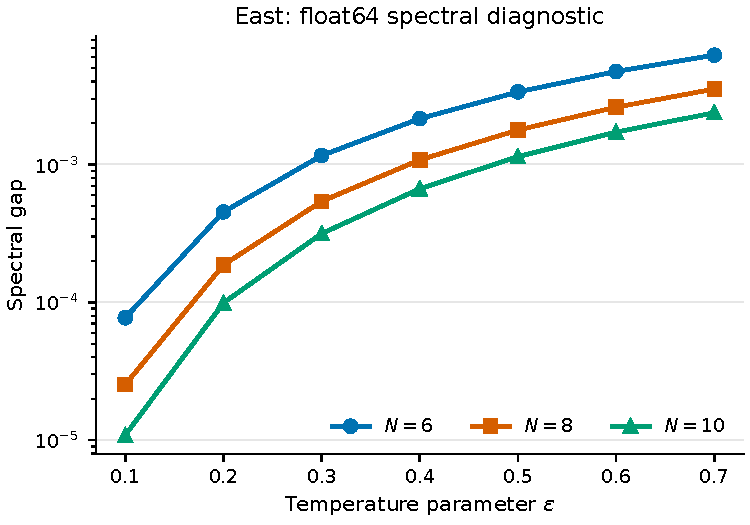
\includegraphics[width=0.7\linewidth]{figures/out/fig_spectral_gaps.pdf}
  \caption{East-model spectral gaps across the declared $(N,\epsilon)$ grid (float64 diagnostic
    used only for window calibration).}
  \label{fig:spectral-gaps}
\end{figure}
